% Created 2014-11-08 Sat 11:30
\documentclass[presentation, bigger]{beamer}
\usepackage[utf8]{inputenc}
\usepackage[T1]{fontenc}
\usepackage{fixltx2e}
\usepackage{graphicx}
\usepackage{longtable}
\usepackage{float}
\usepackage{wrapfig}
\usepackage[normalem]{ulem}
\usepackage{textcomp}
\usepackage{marvosym}
\usepackage{wasysym}
\usepackage{latexsym}
\usepackage{amssymb}
\usepackage{amstext}
\usepackage{hyperref}
\tolerance=1000
\usetheme{kuleuven}
\useinnertheme{rectangles}
\graphicspath{{graphics/}}
\usepackage[style=authoryear,hyperref,backref,square,natbib,ibidtracker=false]{biblatex}
\bibliography{bibliography}
\usepackage[dutch, english]{babel}
\usepackage{graphicx}
\usetheme{default}
\author{Ward Schodts, Xavier Goás Aguililla}
\date{maandag 10 november 2014}
\title{Internet of Things code deployment metrics}
\hypersetup{
  pdfkeywords={},
  pdfsubject={},
  pdfcreator={Emacs 24.3.1 (Org mode N/A)}}
\begin{document}

\maketitle
\begin{frame}{Outline}
\tableofcontents
\end{frame}


\section{Introductie}
\label{sec-1}
\begin{frame}[label=sec-1-1]{Wireless sensor networks: wat zijn ze?}
\begin{itemize}
\item TODO hier een afbeelding zoeken en aan de hand hiervan uitleggen!
\item bestaan uit embedded computers, zgn. ‘motes’
TODO foto/video van motes
\item uitgerust met low-power radioantennes en sensoren
\end{itemize}
\end{frame}

\begin{frame}[label=sec-1-2]{Toepassingen van WSN}

\begin{columns}[t]
\column{.5\textwidth}
\centering
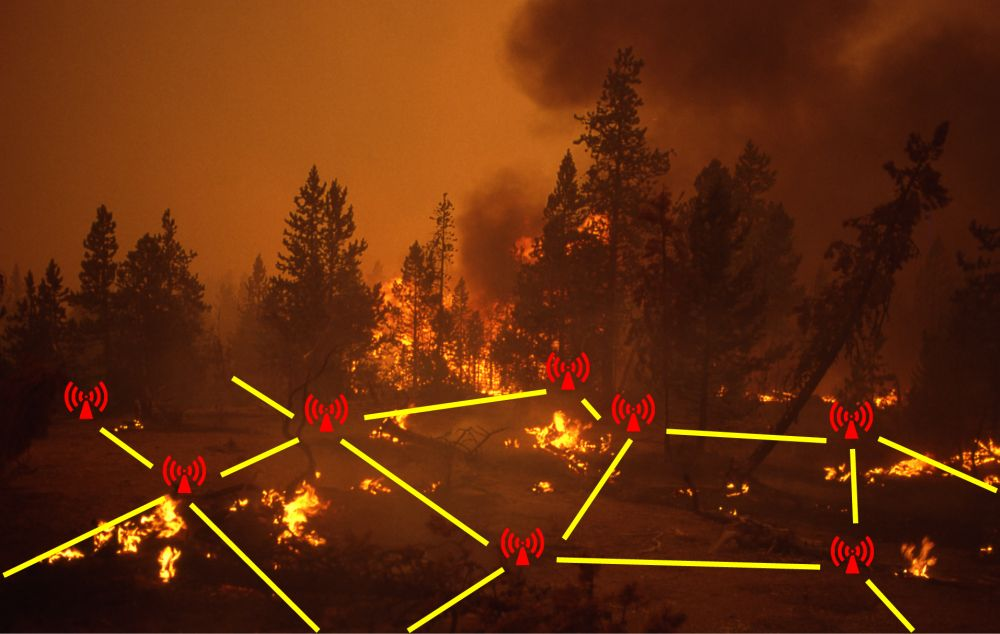
\includegraphics[width=5.25cm,height=3.5cm]{graphics/sample_applications/fire.jpg}\\
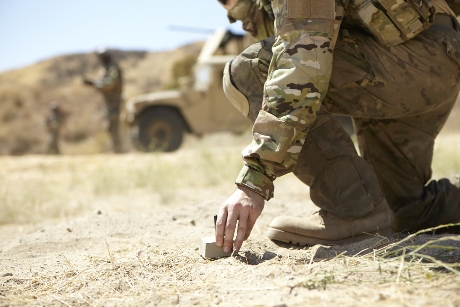
\includegraphics[width=5.25cm,height=3.5cm]{graphics/sample_applications/military.jpg}
\column{.5\textwidth}
\centering
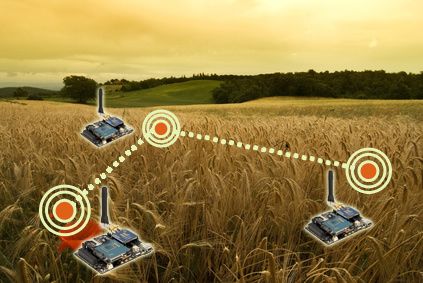
\includegraphics[width=5cm,height=3.5cm]{graphics/sample_applications/landbouw.jpg}\\
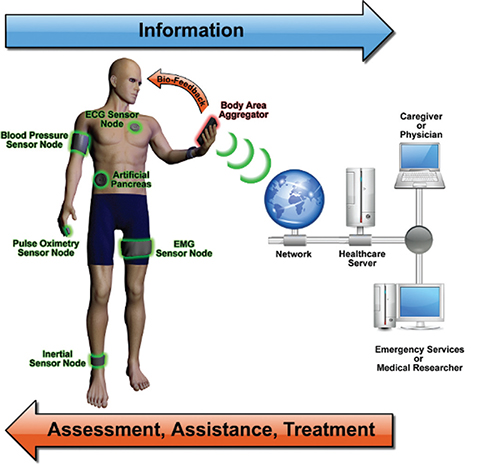
\includegraphics[width=5cm,height=3.5cm]{graphics/sample_applications/medicine.jpg}
\end{columns}
\note{And many more}

\end{frame}

\begin{frame}[label=sec-1-3]{Great Duck Island experiment (1)}

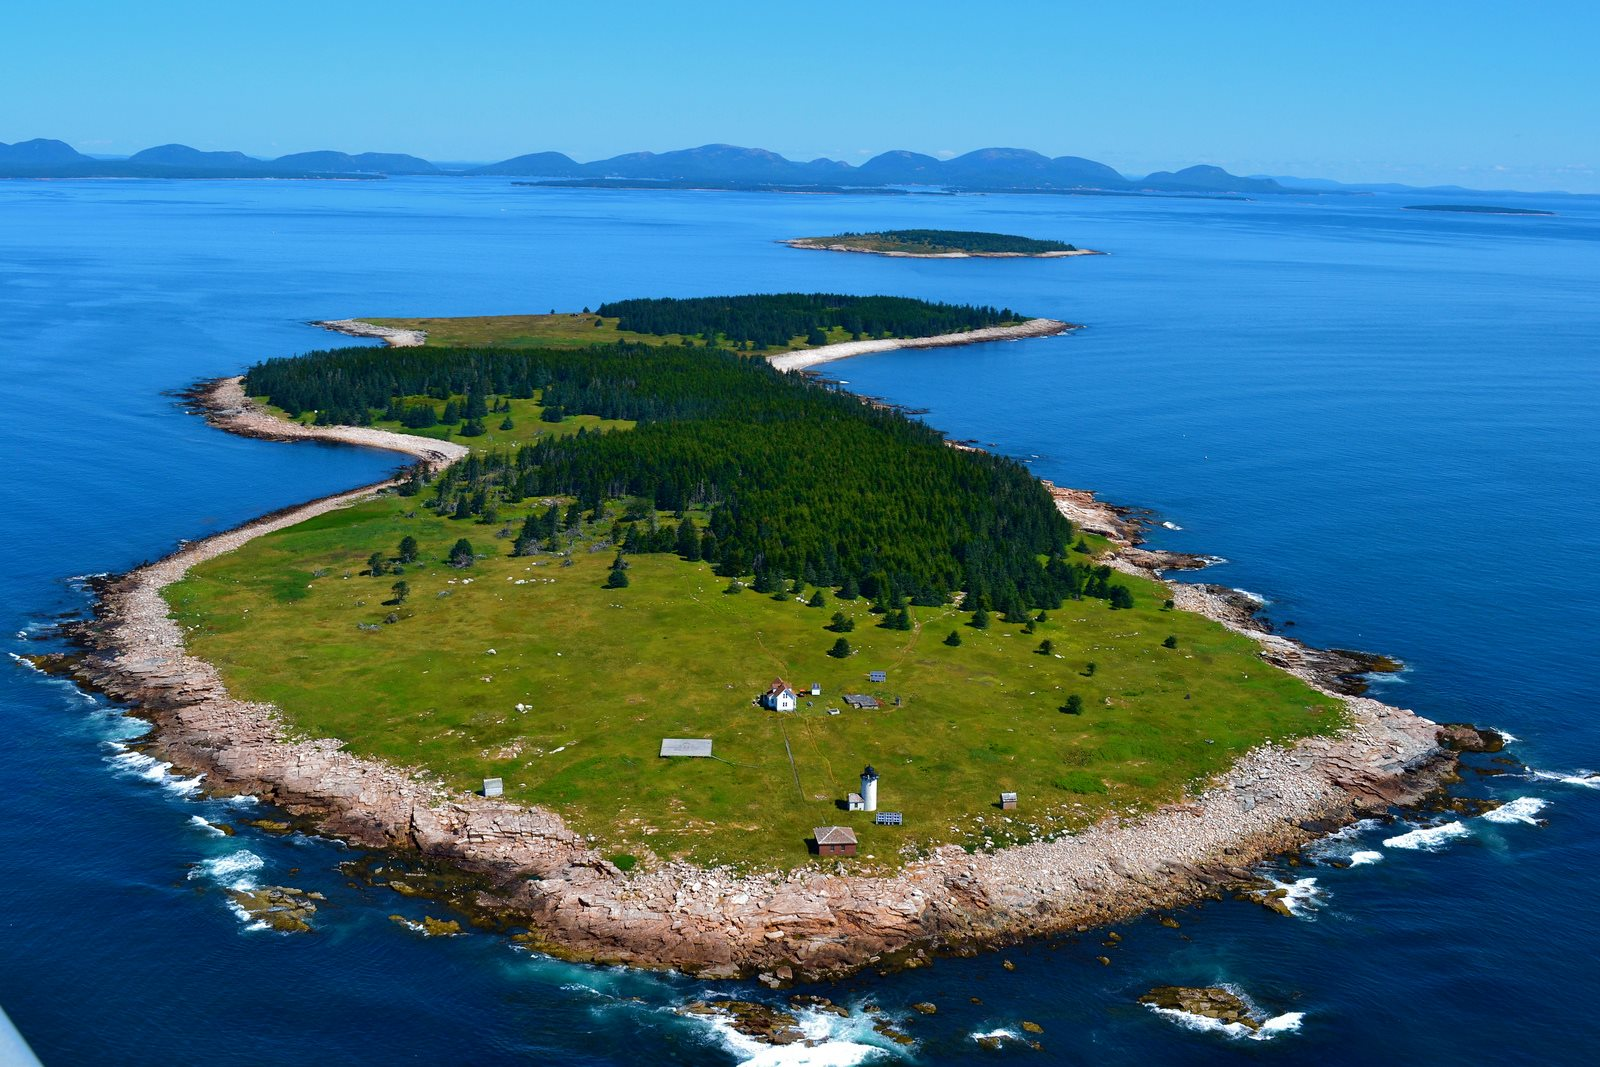
\includegraphics[width=\textwidth,keepaspectration=true]{gdi/gdi.jpg}

\end{frame}

\begin{frame}[label=sec-1-4]{Great Duck Island experiment (2)}
\begin{columns}[t]
\column{.5\textwidth}
\centering
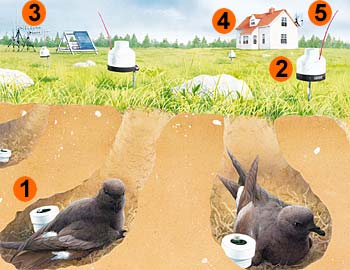
\includegraphics[width=5cm,height=3.5cm]{gdi/gdi_duckmote.jpg}\\
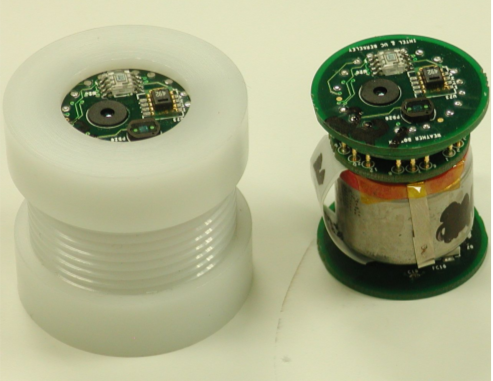
\includegraphics[width=5cm,height=3.5cm]{gdi/gdi_mote.png}
\column{.5\textwidth}
\centering
\begin{itemize}
\item enkele sleutelwoorden hier
\end{itemize}
\end{columns}

\end{frame}
\begin{frame}[label=sec-1-5]{Belangrijke aspecten bij WSN design}
\begin{itemize}
\item energie-efficiëntie
\item robuustheid
\item autonomie
\item TODO verder bij survey paper
\end{itemize}
\end{frame}

\begin{frame}[label=sec-1-6]{Store, compute, transmit? (1)}
\begin{itemize}
\item drie grote factoren in energieverbruik
\begin{itemize}
\item flash-opslag
\item CPU-operaties
\item data-overdracht
\end{itemize}
\item uitleggen dat transmitting het meeste energie verbruikt
\end{itemize}
\end{frame}

\begin{frame}[label=sec-1-7]{Store, compute, transmit? (2)}
\begin{itemize}
\item Mss een grafiekje dat de verschillen duidt?
\item diagram van Hughes tijdens presentatie gebruiken
\end{itemize}
\end{frame}
\section{Middleware voor WSNs}
\label{sec-2}
\begin{frame}[label=sec-2-1]{Wat is middleware?}
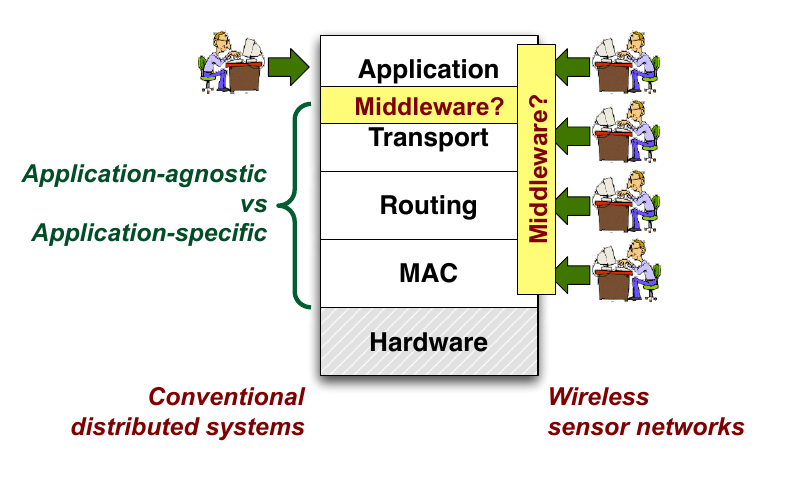
\includegraphics[width=\textwidth,keepaspectration=true]{middleware}
\end{frame}

\begin{frame}[label=sec-2-2]{Mogelijke aanpakken}
\begin{itemize}
\item application-based; bv. Contiki, Squawk
\item component-based; bv. OpenCOM, Figaro, LooCi
\begin{itemize}
\item statisch
\item dynamisch reconfigureerbaar
\end{itemize}
\end{itemize}
\end{frame}

\begin{frame}[label=sec-2-3]{LooCi}
\begin{itemize}
\item Kort historisch
\item Hoe werkt t. (vb vm?)
\end{itemize}
\end{frame}
\section{Energieverbruik analyseren}
\label{sec-3}

\begin{frame}[label=sec-3-1]{Waarom is energiegebruik belangrijk?}
\begin{itemize}
\item WSN-motes moeten lang meegaan
\item energie-efficiëntie is van groot belang
\end{itemize}
\end{frame}

\begin{frame}[label=sec-3-2]{Hoe meten we het?}
\begin{itemize}
\item oscilloscoop
foto/filmpje
\item software-triggers starten metingen
\item stroomverbruik analyseren met de wet van Ohm
\end{itemize}
\end{frame}

\begin{frame}[label=sec-3-3]{Setup}
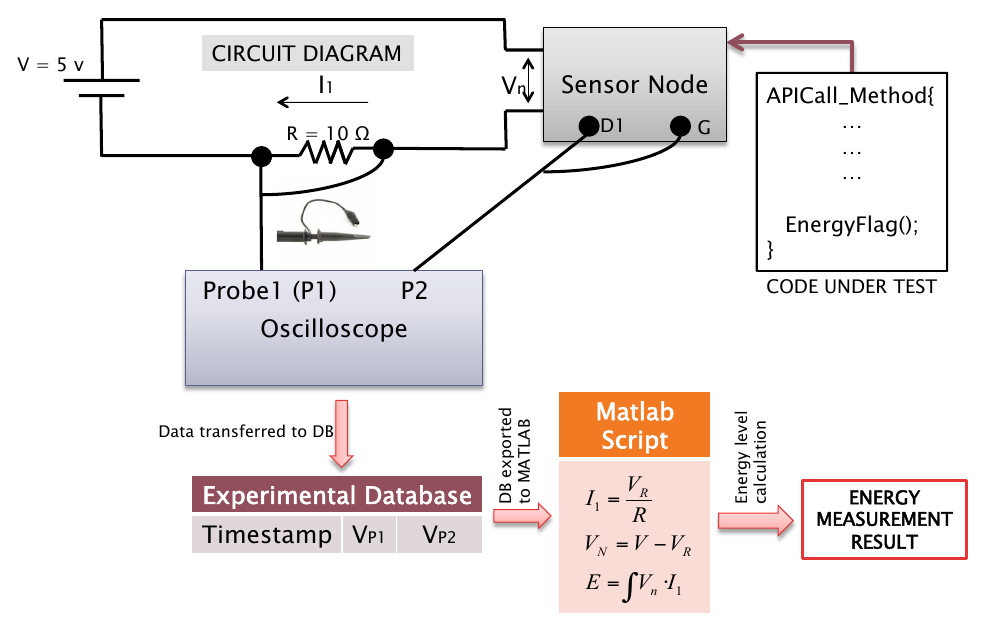
\includegraphics[width=\textwidth,keepaspectration=true]{energy_measurement_diagram}
\end{frame}

\begin{frame}[label=sec-3-4]{Voltageplot}
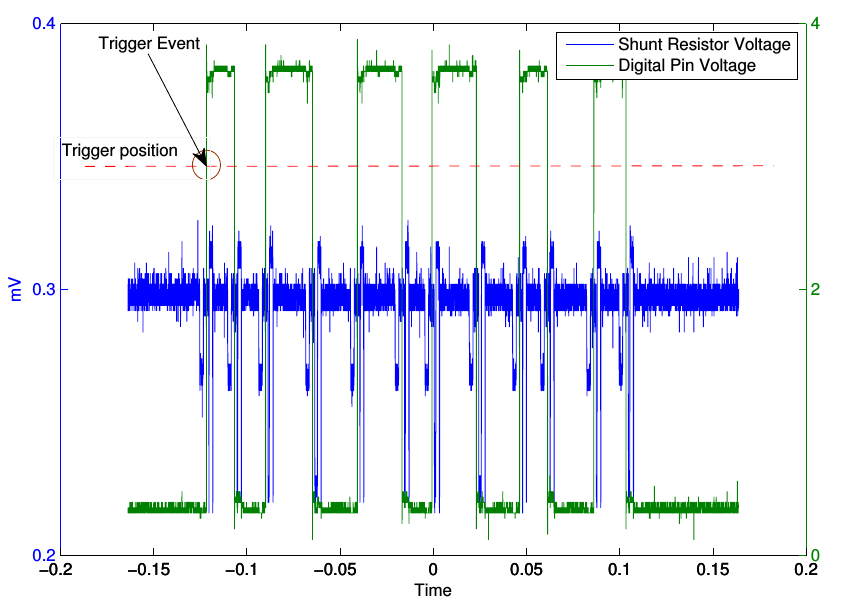
\includegraphics[width=0.95\textwidth,keepaspectration=true]{energy_measurement_plot}
\end{frame}

\begin{frame}[label=sec-3-5]{Analyse energieverbruik}
\begin{itemize}
\item kan afgeleid worden met de wet van Ohm
\item kan gemodeleerd worden m.b.v. lineaire regressie
\end{itemize}
\end{frame}
\section{Conclusie}
\label{sec-4}
\begin{frame}[label=sec-4-1]{Waar komen wij in het spel?}
\begin{itemize}
\item huidige aanpak in het veld: netwerk-overdracht
\item is dit wel zo?
\item implementeren tool voor simulatie energieverbruik
\end{itemize}
\end{frame}

\begin{frame}[label=sec-4-2]{Conclusie}
\end{frame}
\begin{frame}[label=sec-4-3]{Bibliografie}
\nocite{*}
\printbibliography
\end{frame}
% Emacs 24.3.1 (Org mode N/A)
\end{document}
